\section{Dynamic Programming}

The key idea of Dynamic Programming in Reinforcement Learning is to use an iteratice process to change the values of the value functions to improve the policy. The process is called \textit{Generalized Policy Iteration}.

\subsection{Policy Iteration}

\subsection{Policy Evaluation (Prediction)}

Policy Evaluation uses the equation of the Bellman Expectation Equation to estimate the value function of a policy. The Bellman Expectation Equation is given by

\begin{equation}
    v_\pi(s) = \sum_a \pi(a\mid s)\sum_{s',r}p(s',r\mid s,a)\left[r + \gamma v_\pi(s')\right]
\end{equation}where $v_\pi(s)$ is the probability of taking the action a in the state s, following the policy $\pi$.

The policy evaluation finds the optimal value function of a policy by solving the Bellman Expectation Equation iteratively. The algorithm is given by

\begin{algorithm}[H]
    \caption{Policy Evaluation}
    \begin{algorithmic}[1]
        \State Input $\pi$, the policy to be evaluated
        \State Algorithm parameter: a small threshold $\theta>0$ determining accuracy of estimation
        \State Initialize $V(s)$ arbitrarily, for $s\in\mathcal{S}$, and $V(terminal)$ to $0$
        \Repeat
            \State $\Delta \leftarrow 0$
            \For{each $s\in\mathcal{S}$}
                \State $v \leftarrow V(s)$
                \State $V(s) \leftarrow \sum_a \pi(a\mid s)\sum_{s',r}p(s',r\mid s,a)\left[r + \gamma V(s')\right]$
                \State $\Delta \leftarrow \max(\Delta, |v-V(s)|)$
            \EndFor
        \Until{$\Delta < \theta$}
    \end{algorithmic}
\end{algorithm}

The policy evaluation algorithm, when used on a simple $4\times 4$ grid world, converges to the optimal value function of the policy.

\subsubsection{Policy Improvement}

Policy Improvement is choosing the best action in each state greedily by choosing the action that maximizes the value function.

It follows from the idea that, if you select an action $a$ from $s$ and then follow the policy $\pi$ and the return turned out to be better than all other actions, then it is better to choose the action $a$ from the state $s$ always.

Let the improved policy is $\pi'$, if for all $s\in \mathcal{S}$, $q_\pi(s, \pi'(s)) \geq v_\pi(s)$. Then the policy $\pi'$ is better than or equal to the policy $\pi$.

\begin{equation}
    \pi'(s) \doteq \argmax_a q_\pi(s, a) 
\end{equation}

\begin{equation}
    v_{\pi'}(s) = \max_a \sum_{s',r}p(s',r\mid s,a)\left[r + \gamma v_{\pi'}(s')\right]
\end{equation}

\subsubsection{Policy Iteration}

Once a policy has been evaluated and improved, the process is repeated until the policy cenverges to the optimal policy. This process is called Policy Iteration. We can show it as:

\begin{equation}
    \pi_0 \xrightarrow{E} v_{\pi_0} \xrightarrow{I} \pi_1 \xrightarrow{E} v_{\pi_1} \xrightarrow{I} \pi_2 \xrightarrow{E} \cdots \xrightarrow{I} \pi_\ast \xrightarrow{E} v_\ast
\end{equation}

The policy iteration algorithm is given by

\begin{algorithm}[H]
    \caption{Policy Iteration}
    \begin{algorithmic}
        \State Initialization:
        \State $V(s)\in \mathbb{R}$ and $\pi(s)\in \mathcal{A}(s)$ arbitrarily for all $s\in \mathcal{S}$; $V(terminal) \doteq 0$
        \State
    \end{algorithmic}
    \begin{algorithmic}
        \State Policy Evaluation:
        \Repeat
            \State $\Delta \leftarrow 0$
            \For{each $s\in \mathcal{S}$}
                \State $v \leftarrow V(s)$
                \State $V(s) \leftarrow \sum_{s',r}p(s',r\mid s,\pi(s))\left[r + \gamma V(s')\right]$
                \State $\Delta \leftarrow \max(\Delta, |v-V(s)|)$
            \EndFor
        \Until{$\Delta < \theta$}
        \State
    \end{algorithmic}
    \begin{algorithmic}
        \State Policy Improvement:
        \State $policy\_stable \leftarrow true$
        \For{each $s\in \mathcal{S}$}
            \State $old\_action \leftarrow \pi(s)$
            \State $\pi(s) \leftarrow \argmax_a \sum_{s',r}p(s',r\mid s,a)\left[r + \gamma V(s')\right]$
            \If{$old\_action \neq \pi(s)$}
                \State $policy\_stable \leftarrow false$
            \EndIf
        \EndFor
        \If{$policy\_stable$}
            \Return $\pi$ and $V$
            \State \textbf{break}
        \Else
            \State \textbf{go to Policy Evaluation}
        \EndIf
    \end{algorithmic}
\end{algorithm}

\subsection{Jack's Car Rental Problem}

Jack manages two locations for a nationwide car rental company. Each day, some number of customers arrive at each location to rent cars. If Jack has a car available, he rents it out and is credited $\$10$ by the national company. If he is out of cars at that location, then the business is lost. Cars become available for renting the day after they are returned. To help ensure that cars are available where they are needed, Jack can move them between the two locations overnight, at a cost of $\$2$ per car moved. We assume that the number of cars requested and returned at each location are Poisson random variables, meaning that the probability that the number is $\frac{\lambda^n}{n!}e^{-\lambda}$, where is the expected number. Suppose is 3 and 4 for rental requests at the first and second locations and 3 and 2 for returns. To simplify the problem slightly, we assume that there can be no more than 20 cars at each location (any additional cars are returned to the nationwide company, and thus disappear from the problem) and a maximum of five cars can be moved from one location to the other in one night. We take the discount rate to be = 0.9 and formulate this as a continuing finite MDP, where the time steps are days, the state is the number of cars at each location at the end of the day, and the actions are the net numbers of cars moved between the two locations overnight.

Policy Iteration is used to solve the Jack's Car Rental Problem. The policy evaluation is done using the Bellman Expectation.

The results obtained from the Policy Iteration are shown in the figure~\ref{fig:jack-car-rental}.

\begin{figure}[h!]
    \centering
    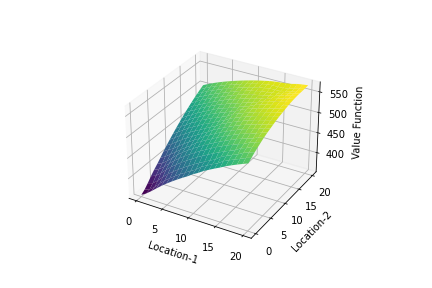
\includegraphics[width=0.49\textwidth]{images/jack-1-3d.png}
    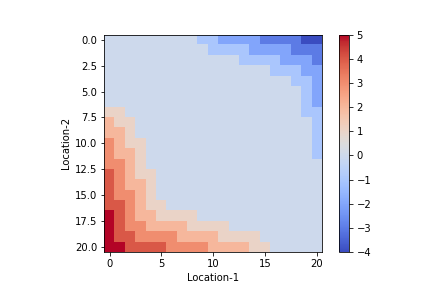
\includegraphics[width=0.49\textwidth]{images/jack-1-pi.png}
    \caption{The results obtained from the Policy Iteration of the Jack's Car Rental Problem.}
    \label{fig:jack-car-rental}
\end{figure}

If the following modifications are made to the Jack's Car Rental Problem:

\begin{figure}[h!]
    \centering
    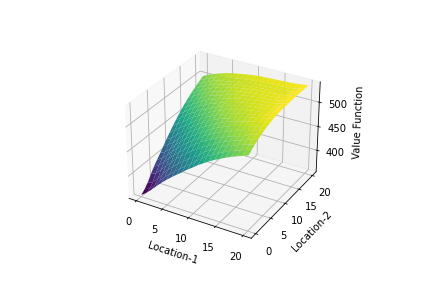
\includegraphics[width=0.49\textwidth]{images/jack-2-3d.png}
    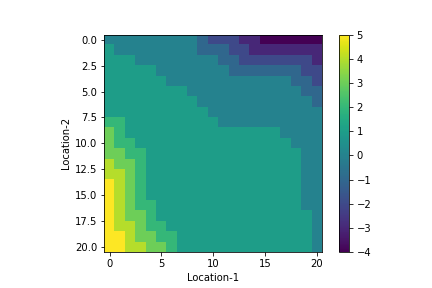
\includegraphics[width=0.49\textwidth]{images/jack-2-pi.png}
    \caption{The results obtained from the Policy Iteration of the Jack's Car Rental Problem with the modifications.}
    \label{fig:jack-car-rental-modified}
\end{figure}

The results obtained from the Policy Iteration of the Jack's Car Rental Problem with the modifications are shown in the figure~\ref{fig:jack-car-rental-modified}.

The values represented in the right side of the figures in the number of cars to be moved from the first locaation to the second location to get the maximum returns.

\subsection{Gambler's Problem}

A gambler has the opportunity to make bets on the outcomes of a sequence of coin flips. If the coin comes up heads, he wins as many dollars as he has staked on that flip; if it is tails, he loses his stake. The game ends when the gambler wins by reaching his goal of \$100, or loses by running out of money. On each flip, the gambler must decide what portion of his capital to stake, in integer numbers of dollars. This problem can be formulated as an undiscounted, episodic, finite MDP. The state is the gambler's capital, $s \in \{1, 2, . . . , 99\}$ and the actions are stakes, $a \in {0, 1, . . . , \min(s, 100-s)}$. The reward is zero on all transitions except those on which the gambler reaches his goal, when it is +1. The state-value function then gives the probability of winning from each state. A policy is a mapping from estimates levels of capital to stakes. The optimal policy maximizes the probability of reaching the goal. Let $p_h$ denote the probability of the coin coming up heads. If ph is known, then the entire problem is known and it can be solved, for instance, by value iteration.

I tried the Policy Iteration to solve the Gambler's Problem for $p_h=0.40$, $p_h=0.25$, $p_h=0.55$, and $p_h=0.50$. 

\begin{figure}[h!]
    \centering
    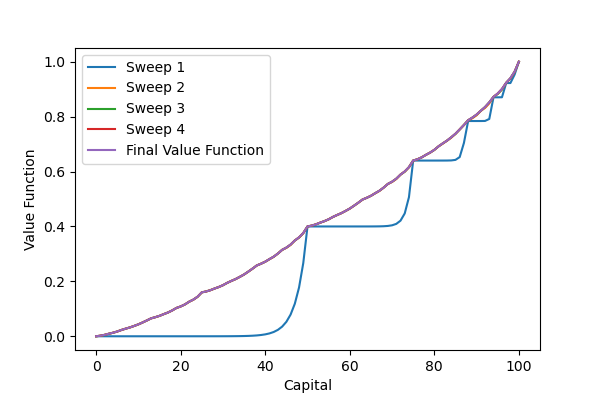
\includegraphics[width=0.49\textwidth]{images/sweeps-0.4.png}
    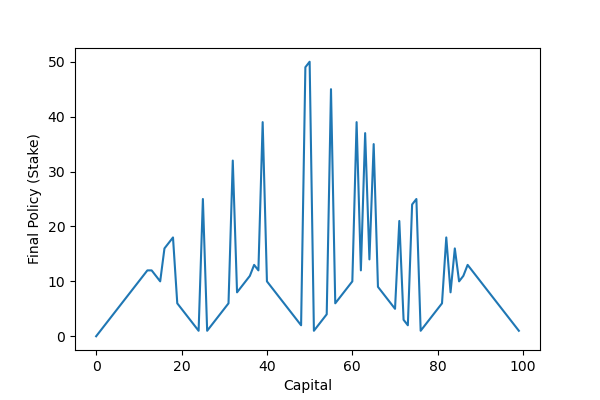
\includegraphics[width=0.49\textwidth]{images/pi-0.4.png}
    \caption{The results obtained from the Policy Iteration of the Gambler's Problem for $p_h=0.40$.}
    \label{fig:gambler-0.40}
\end{figure}

\begin{figure}[h!]
    \centering
    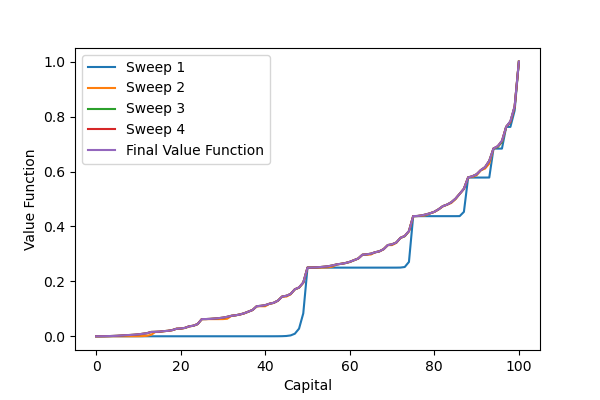
\includegraphics[width=0.49\textwidth]{images/sweeps-0.25.png}
    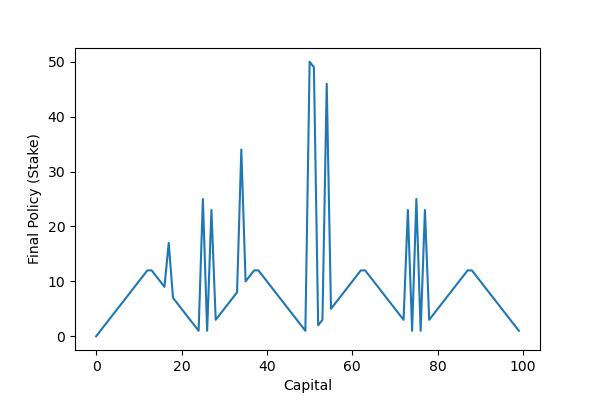
\includegraphics[width=0.49\textwidth]{images/pi-0.25.png}
    \caption{The results obtained from the Policy Iteration of the Gambler's Problem for $p_h=0.25$.}
    \label{fig:gambler-0.25}
\end{figure}

\begin{figure}[h!]
    \centering
    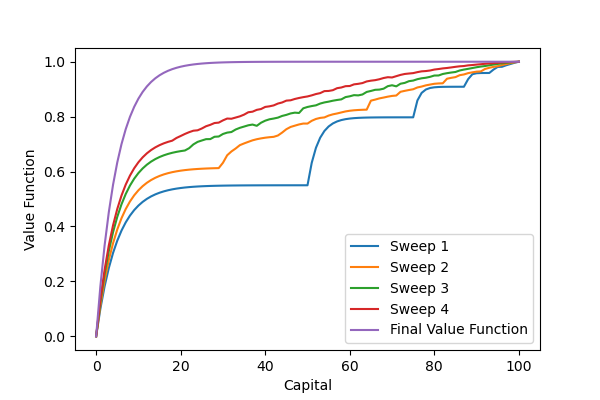
\includegraphics[width=0.49\textwidth]{images/sweeps-0.55.png}
    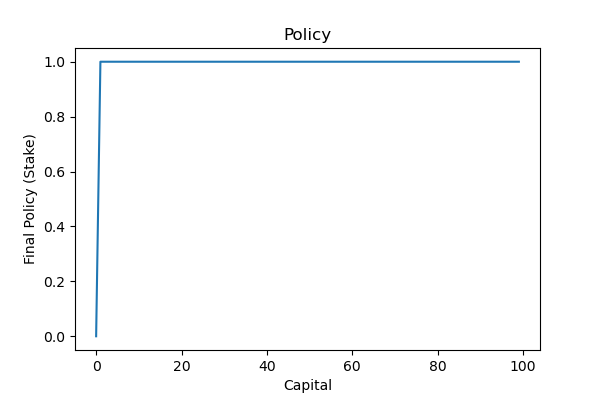
\includegraphics[width=0.49\textwidth]{images/pi-0.55.png}
    \caption{The results obtained from the Policy Iteration of the Gambler's Problem for $p_h=0.55$.}
    \label{fig:gambler-0.55}
\end{figure}

\begin{figure}[h!]
    \centering
    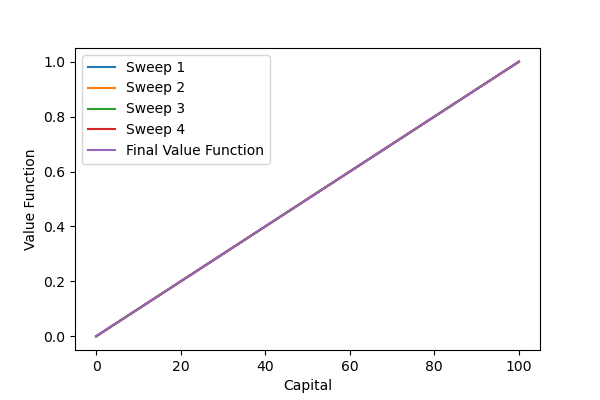
\includegraphics[width=0.49\textwidth]{images/sweeps-0.5.png}
    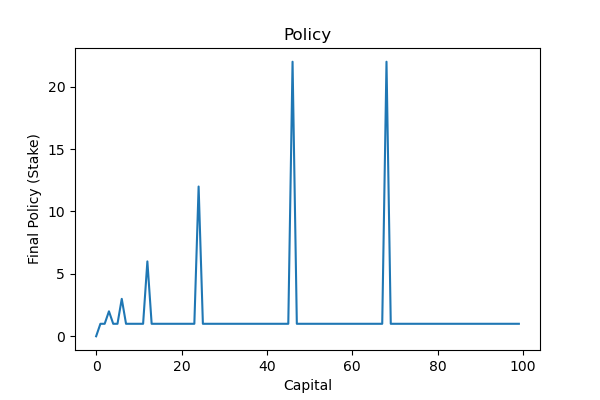
\includegraphics[width=0.49\textwidth]{images/pi-0.5.png}
    \caption{The results obtained from the Policy Iteration of the Gambler's Problem for $p_h=0.50$.}
    \label{fig:gambler-0.50}
\end{figure}

Of course, the most beautiful graph is the one with $p_h=0.55$. As expected, when $p_h \geq 0.50$, the engine tries to set the stake as just 1, because the expected value is positive and the maximum loss is minimised. This was something I learnt, because I would never use such a strategy myself. The regularities in the graphs for $p_h=0.40$ and $p_h=0.25$ are also interesting.